\documentclass[a4paper,fontsize=12]{report}
  \usepackage[left=1.5cm,right=1.5cm,
      top=1.5cm,bottom=2cm,bindingoffset=0cm]{geometry}
  \usepackage{scrextend}
  \usepackage[T1,T2A]{fontenc}
  \usepackage[utf8]{inputenc}
  \usepackage[english,russian,ukrainian]{babel}
  \usepackage{tabularx}
  \linespread{1.3}
  \usepackage{amssymb}
  \usepackage{color}
  \usepackage{amsmath}
  \usepackage{mathrsfs}
  \usepackage{listings}
  \usepackage{graphicx}
  \usepackage{lipsum}
  \usepackage{xcolor}
  \usepackage{hyperref}
  \usepackage{tcolorbox}
  \usepackage{tikz}
  \usepackage[framemethod=TikZ]{mdframed}
  \usepackage{wrapfig,boxedminipage,lipsum}
   \usepackage{csvsimple}
   \usepackage{supertabular}
  \usepackage{pdflscape}
  \usepackage{fancyvrb}
  %\usepackage{comment}
  \usepackage{array,tabularx}
  \usepackage{colortbl}

  \usepackage{varwidth}
  \tcbuselibrary{skins}
  \usepackage{fancybox}
  \usepackage{spreadtab}


  \usepackage{tikz}
  \usepackage[framemethod=TikZ]{mdframed}
  \usepackage{xcolor}
  \usetikzlibrary{calc}
  \makeatletter
  \newlength{\mylength}
  \xdef\CircleFactor{1.1}
  \setlength\mylength{\dimexpr\f@size pt}
  \newsavebox{\mybox}
  \newcommand*\circled[2][draw=blue]{\savebox\mybox{\vbox{\vphantom{WL1/}#1}}\setlength\mylength{\dimexpr\CircleFactor\dimexpr\ht\mybox+\dp\mybox\relax\relax}\tikzset{mystyle/.style={circle,#1,minimum height={\mylength}}}
  \tikz[baseline=(char.base)]
  \node[mystyle] (char) {#2};}
  \makeatother
   % Цвета для гиперссылок
  \definecolor{linkcolor}{rgb}{0.6, 0.4, 0.8} % цвет ссылок
  \definecolor{urlcolor}{rgb}{0.0, 0.0, 1.0}% цвет гиперссылок
  \hypersetup{pdfstartview=FitH,  linkcolor=linkcolor,urlcolor=urlcolor,citecolor=red, colorlinks=true}

  \definecolor{ggreen}{rgb}{0.4,1,0}
  \definecolor{rred}{rgb}{1,0.1,0.1}
  \definecolor{amber}{rgb}{1.0, 0.75, 0.0}
  \definecolor{babyblue}{rgb}{0.54, 0.81, 0.94}
  \definecolor{amethyst}{rgb}{0.6, 0.4, 0.8}

\usepackage[backend=biber,style=numeric,sorting=none]{biblatex}
\usepackage{csquotes}
\addbibresource{books.bib} %% подключение библиографической базы из файла sample.bib

\begin{document}



\renewcommand{\bibname}{Список використаної літератури}
\newcommand{\myimage}[4]{%
\center{\includegraphics[width=#1\linewidth]{#2}}
\caption{#3}\label{#4}}%

%\pagecolor{white}

%----------------------------------------1
\newtcbox{\xmybox}[1][red]{on line, arc=7pt,colback=#1!10!white,colframe=#1!50!black, before upper={\rule[-3pt]{0pt}{10pt}},boxrule=1pt, boxsep=0pt,left=6pt,right=6pt,top=2pt,bottom=2pt}

\begin{titlepage}
  \begin{center}
  \large
  Національний технічний університет України \\ "Київський політехнічний інститут імені Ігоря Сікорського"


  
  Факультет Електроніки

  Кафедра мікроелектроніки
  \vfill

  \textsc{РЕФЕРАТ}\\

  %{\Large Про виконання лабораторної роботи №1\\
  з дисципліни: «Фізичні основи сенсорики»\\[1cm]

  Тактильні сенсори


  %}
  \bigskip
  \end{center}
  \vfill

  \newlength{\ML}
  \settowidth{\ML}{«\underline{\hspace{0.4cm}}» \underline{\hspace{2cm}}}
  \hfill
  \begin{minipage}{1\textwidth}
  Виконавець:\\
  Студент 4-го курсу \hspace{4cm} $\underset{\text{(підпис)}}{\underline{\hspace{0.2\textwidth}}}$  \hspace{1cm}Мнацаканов А. С.\\
  \vspace{1cm}

  Перевірила: \hspace{5.6cm} $\underset{\text{(підпис)}}{\underline{\hspace{0.2\textwidth}}}$  \hspace{1cm}доц. Коваль В. М.\\

  \end{minipage}

  \vfill

  \begin{center}
  2021
  \end{center}
\end{titlepage}

\tableofcontents
\setcounter{page}{2}
\newpage

\chapter{Ємнісні датчики дотику}
  Протягом останнього десятиліття або близько того стало дійсно важко уявити собі світ з електронікою без сенсорних датчиків дотиків. Смартфони є тому найбільш помітним і поширеним прикладом, але, звичайно, існують і інші численні пристрої та системи, які мають датчиками дотиків. Для побудови сенсорних датчиків дотиків можуть використовуватися і ємність, і опір; в даному розділі ми будемо обговорювати тільки ємнісні датчики, які є кращими в реалізації.\\

  Хоча застосування, засновані на ємнісних датчиках, можуть бути досить складними, фундаментальні принципи, що лежать в основі даної технології, досить прості. Насправді, якщо ви розумієте суть ємності і фактори, які визначають ємність конкретного конденсатора, ви стоїте на правильному шляху в розумінні роботи ємнісних сенсорних датчиків дотику.\\

  Ємнісні сенсорні датчики дотику діляться на дві основні категорії: на основі взаємної ємності і на основі власної ємності. Перший з них, в якому конденсатор датчика складається з двох виводів, які діють як випромінюючий і приймальний електроди, є більш прийнятним для сенсорних дисплеїв. Останній, в якому один вивід конденсатора датчика підключений до землі, є прямим підходом, який підходить для сенсорної кнопки, слайдера або колеса. В даному розділі ми розглянемо датчики на основі власної ємності.\\
\section{Конденсатор на базі друкованої плати}\par

  Конденсатори можуть бути різних типів. Ми всі звикли бачити ємність у вигляді компонентів з виводами або корпусів поверхневого монтажу, але насправді, все, що вам дійсно необхідно, це два провідника, розділених ізолюючим матеріалом (тобто діелектриком). Таким чином, досить просто створити конденсатор, використовуючи лише електропровідні шари, розділені друкованою платою. Наприклад, розглянемо наступні вид зверху і вид збоку друкованого конденсатора, що використовується в якості сенсорної кнопки дотику (зверніть увагу на перехід на інший шар друкованої плати на малюнку виду збоку).

  \begin{figure}[h]
  \myimage{0.7}{1.jpeg}{Cенсорна кнопка}{i1}
  \end{figure}


  Ізолюючий поділ між сенсорною кнопкою і міддю створює конденсатор. В цьому випадку, навколишнє мідь підключена до землі, і, отже, наша сенсорна кнопка може бути змодельована, як конденсатор між сенсорної сигнальної майданчиком і землею.\\

  Можливо, зараз ви захочете дізнатися, яку ємність реально забезпечує така розводка друкованої плати. Крім того, як ми розрахуємо її точно? Відповідь на перше питання: ємність дуже мала, може становити близько 10 пФ. Що стосується другого питання: не хвилюйтеся, якщо забули електростатики, тому що точне значення ємності конденсатора не має ніякого значення. Ми шукаємо тільки зміни в ємності, і ми можемо виявити ці зміни без знання номінального значення ємності друкованого конденсатора.\\
\section{Вплив пальця}

  Так що ж викликає ці зміни ємності, які контролер датчика дотиків збирається виявити? Ну, звичайно ж, людський палець.

  \begin{figure}[h]
  \myimage{0.6}{2.jpeg}{Вплив пальця на сенсорну кнопку}{i2}
  \end{figure}
  Перш, ніж ми обговоримо, чому палець змінює ємність, важливо розуміти, що тут немає прямого електричного контакту; палець ізольований від конденсатора лаком на друкованій платі і, як правило, шаром пластика, який відокремлює електроніку пристрою від зовнішнього середовища. Так що палець не розряджає конденсатор, і, крім того, кількість заряду, що зберігається в конденсаторі в певний момент, не представляє інтересу - скоріше інтерес представляє ємність в певний момент.\\

  Отже, чому ж присутність пальця змінює ємність? Є дві причини: перша включає в себе діелектричні властивості пальця, а друга включає в себе його провідні властивості.
\section{Палець як діелектрик}

  Зазвичай ми думаємо про конденсаторі, як має фіксовану величину, яка визначається площею двох провідних пластин, відстанню між ними і діелектричної проникністю матеріалу між пластинами. Ми, звичайно, не можемо змінити фізичні розміри конденсатора, просто доторкнувшись до нього, але ми можемо змінити діелектричну проникність, так як палець людини має діелектричні характеристиками, відмінними від матеріалу (імовірно повітря), який він витісняє. Це правда, що палець не буде знаходитися в цій області діелектрика, тобто в ізолюючому просторі безпосередньо між провідниками, але таке «вторгнення» в конденсатор необов'язково:

  \begin{figure}[h]
  \myimage{0.6}{3.jpeg}{Вплив пальця на сенсорну кнопку в якості діелектрика}{i3}
  \end{figure}

  Як показано на малюнку, щоб змінити діелектричні характеристики, немає необхідності поміщати палець між пластинами, оскільки електричне поле конденсатора поширюється в навколишнє середовище.\\

  Виявляється, що людська плоть є досить хорошим діелектриком, тому що наші тіла складаються в основному з води. Відносна діелектрична проникність вакууму дорівнює 1, а відносна діелектрична проникність повітря лише трохи вище (близько 1,0006 на рівні моря при кімнатній температурі). Відносна діелектрична проникність води набагато вище, близько 80. Таким чином, взаємодія пальця з електричним полем конденсатора являє собою збільшення відносної діелектричної проникності, і, отже, призводить до збільшення ємності.
\section{Палець як провідник}
  Той, хто випробував на собі удар електричного струму, знає, що шкіра людини проводить струм. Я вже згадував вище, що прямого контакту між пальцем і сенсорною кнопкою (тобто ситуації, коли палець розряджає друкований конденсатор) немає. Проте, це не означає, що провідність пальця не має значення. Вона насправді дуже важлива, так як палець стає другою провідною пластиною в додатковому конденсаторі:

  \begin{figure}[h]
  \myimage{0.6}{4.jpeg}{Вплив пальця на сенсорну кнопку в якості провідника}{i4}
  \end{figure}

  На практиці ми можемо припустити, що цей новий конденсатор, створений пальцем, підключений паралельно існуючому друкованого конденсатору. Ця ситуація трохи складніше, тому що людина, що використовує сенсорний пристрій, електрично з'єднаний з землею на друкованій платі, і, таким чином, ці два конденсатора не включені паралельно в звичайному для аналізу ланцюгів сенсі.\\

  Проте, ми можемо думати про людське тіло, як про що забезпечує віртуальну землю, оскільки воно має відносно велику ємність, щоб поглинати електричний заряд. У будь-якому випадку, нам не потрібно турбуватися про точну електричного зв'язку між конденсатором з пальцем і друкованим конденсатором; важливим моментом є те, що псевдопараллельное поєднання цих двох конденсаторів означає, що палець буде збільшувати загальну ємність, так як конденсатор додається паралельно.\\

  Таким чином, ми можемо побачити, що обидва механізми впливу при взаємодії пальця і ємнісного датчика дотику сприяють збільшенню ємності.
\section{Близька відстань або контакт?}
  
  Попереднє обговорення приводить нас до цікавої особливості ємнісних датчиків торкань: вимірюється зміна ємності може бути викликано не тільки контактом між пальцем і датчиком, але і близьким відстанню між ними. Я зазвичай думаю про сенсорному пристрої, як про заміну механічного перемикача або кнопки, але місткість технологія датчиків торкань насправді являє собою новий рівень функціональності, дозволяючи системі визначати відстань між датчиком і пальцем.\\

  Обидва механізми зміни ємності, описані вище, впливають, яке залежить від відстані. Для механізму на базі діелектричної проникності кількість «м'ясного» діелектрика взаємодія з електричним полем конденсатора збільшується при наближенні пальця до провідних частин друкарського конденсатора. Для механізму на базі провідних властивостей ємність конденсатора з пальцем (як і будь-якого іншого конденсатора) обернено пропорційна відстані між провідними пластинами.\\

  Майте на увазі, що цей методу не підходить для вимірювання абсолютного відстані між датчиком і пальцем; ємнісні датчики не пропонують тих даних, які необхідні для виконання точних обчислень абсолютних відстаней. Я вважаю, що можна було б відкалібрувати емкостную сенсорну систему для грубих вимірів відстаней, але так як схема ємнісних датчиків була розроблена для виявлення зміни ємностей, то це означає, що ця технологія особливо підходить для виявлення зміни в відстанях, тобто коли палець наближається або віддаляється від датчика.

\chapter{Індуктивні сенсори дотику}
  %https://www.allaboutcircuits.com/news/how-to-use-inductive-touch-sensors-tis-new-development-board-gives-a-needed/
  На відміну від ємнісного сенсорного сенсора, для якого потрібен лише конденсатор друкованої плати (і кінчик пальця), індуктивний сенсорний дотик включає два окремі компоненти: індуктор друкованої плати та металеву пластину.\\
  \begin{figure}[ht]
    \myimage{1}{6.png}{Cенсор включає в себе два окремих компонента: індуктор PCB і металеву пластину.}{im6}
  \end{figure}
  Схема контролера приводить струм змінного струму в індуктор. Це створює магнітне поле змінного струму, яке створює вихрові струми в провідній пластині. Магнітні поля, що генеруються цими вихровими струмами, взаємодіють з індуктором таким чином, щоб зменшити ефективну індуктивність. Сила взаємодії залежить від відстані між пластиною та індуктором; якщо при натисканні пальцем металева пластина відхиляється, зменшена відстань між пластиною та індуктором призводить до вимірюваної зміни індуктивності.

  Схеми, необхідні для реалізації індуктивного дотику, можна порівняти з тим, що вам потрібно для ємнісного сенсорного сенсора: перетворювач індуктивності в цифровий (LDC) та мікроконтролер. LDC вимірює індуктивність та перетворює її у двійкові дані, які можуть бути оброблені мікроконтролером, який інтерпретує зміни індуктивності та ініціює відповідні відповіді.

  \begin{figure}[h]
  \center{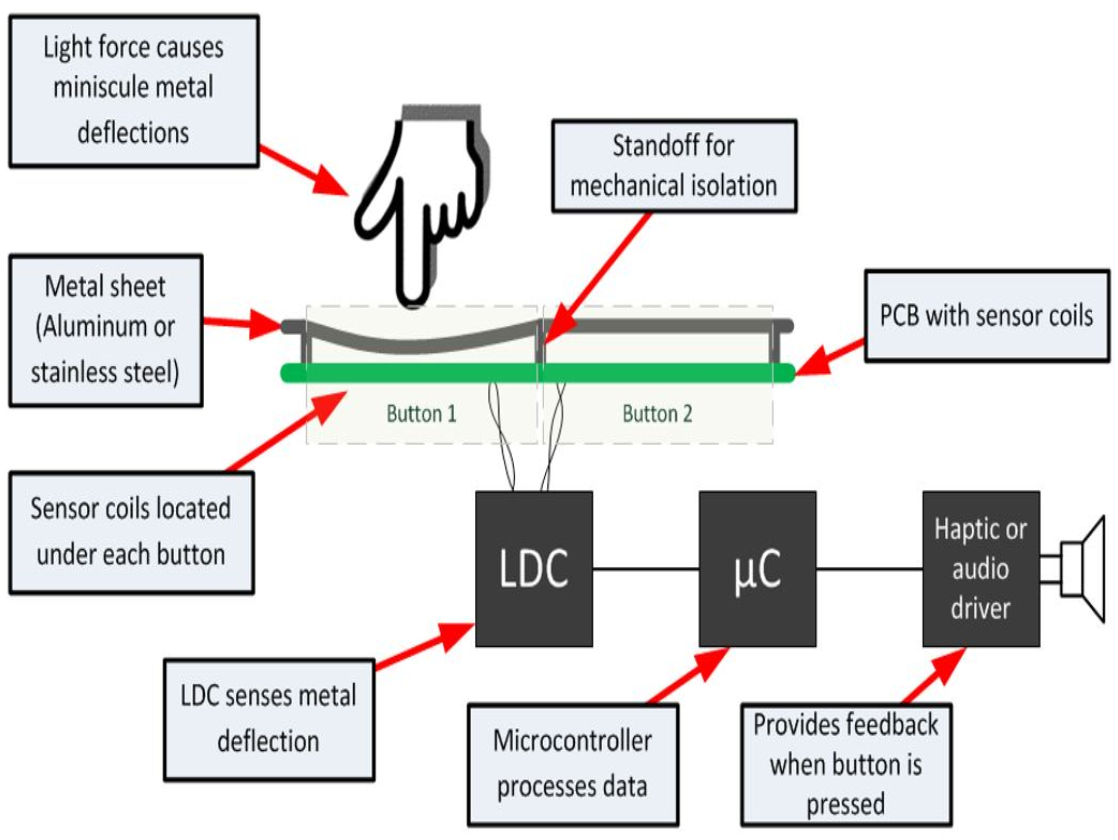
\includegraphics[width=16 cm, height= 9cm]{5.png}}
  \end{figure}

  Я не експерт, але, схоже, основна перевага перед ємнісним сенсором - це стійкість до навколишнього середовища. Різні фактори можуть впливати на ємність сенсора з сенсорним ковпачком-температура, пил, волога. Система індуктивного дотику відчувається більш сумісною з додатками, які вимагають стійкості до несприятливих умов навколишнього середовища.
\chapter{Фотоелектричний сенсор дотику.}
    Робота цих сенсорів заснована на принципі повного внутрішнього відбиття і зазвичай складається з джерела світла і 
    фотоприймача. Коли змінюється тиск, що прикладається до інтерфейсу, інтенсивність відображення чутливого компонента датчика і частота джерела змінюються відповідно.

\chapter{П'єзорезистивний та пєзоелектричний сенсори дотику.}
\section{Принцип рoботи}
  У п'єзорезистивного датчики знімається зміна електричного опору одного або декількох резисторів, встановлених на мембрані.
  Зміна опору прямо пропорційно деформації, викликаної тиском на мембрану. Резистори з'єднані в ланцюг моста Вітстоуна, який є дуже чутливим способом перетворення невеликих змін в вихідна напруга. \\

  Всі три типи датчиків можуть бути миниатюризировать за допомогою кремнієвих технологій виготовлення і об'єднані з електронікою в мікроелектромеханічні системи (MEMS). Це дозволяє створювати дуже маленькі чутливі елементи і об'єднувати їх з електронікою для формування і зчитування сигналу. \\

  У п'єзоелектричних датчиках використовуються матеріали, такі як кристали кварцу або спеціально розроблена кераміка, які створюють заряд на гранях при додатку тиску. Підсилювач заряду перетворює його в вихідна напруга, пропорційне тиску. Задане зусилля призводить до появи відповідного заряду на чутливому елементі. Однак з часом цей заряд витікає, що означає, що датчик не може бути використаний для вимірювання статичного тиску.\\

  П'єзоелектричні датчики чутливі до змін тиску, тому вихідний сигнал зазвичай розглядається як відносне вимірювання тиску, віднесене до вихідного стану п'єзоелектричного матеріалу.\\

  Також, цікаво що п'єзорезистивні і ємнісні датчики тиску можуть використовуватися для абсолютних, надлишкових, відносних або диференціальних вимірювань. \\
\section{Переваги та недоліки}
 { \begin{itemize}
  \item П'єзорезистивного тензометричні датчики
  Це найбільш ранній і найбільш широко використовуваний тип датчиків тиску.

  \item Проста конструкція означає низьку вартість і довговічність. Датчики надійні і добре пручаються ударам, вібрації і динамічних змін тиску.

  \item Схеми зчитування дуже прості і дозволяють проводити вимірювання з високою роздільною здатністю.

  \item Вихідний сигнал лінійно залежить від тиску, а час відгуку зазвичай становить менше однієї мілісекунди.

  \item Вони можуть використовуватися для широкого діапазону вимірювань тиску від 3 фунтів на квадратний дюйм до приблизно 20 000 фунтів на квадратний дюйм (від 21 кПа до 150 МПа). Вихідний сигнал також стабільний в часі.

  \item Резистивні елементи можуть бути приклеєні до мембрани. Це стандартний метод, який використовується вже давно, але можуть виникнути проблеми з клеєм при високих температурах і надмірному тиску.

  \item В якості альтернативи можна створити тонкоплівкові резистори безпосередньо на мембрані. Вони можуть працювати при більш високих температурах і більше підходять для використання в жорстких умовах навколишнього середовища.

  \item Основним недоліком є те, що датчик повинен бути запитан. Це робить їх непридатними для систем з низьким енергоспоживанням або працюють від батарей. Зменшення розмірів зменшує опір і збільшує споживання енергії.

  \item Існують також обмеження на масштабування, оскільки усереднення деформації знижує чутливість датчика. Однак дуже маленькі датчики можуть бути виготовлені у вигляді МЕМС-пристроїв.

  \item Вихідний сигнал датчика залежить від температури. Це може бути великим недоліком для таких додатків, як вимірювання тиску в шинах, де температура сильно змінюється протягом робочого циклу.

  \item Кремнієві тензодатчики набагато більш чутливі і можуть вимірювати тиск до 2 кПа.

  \item Точність МЕМС-пристроїв може бути знижена струмом витоку через спаї. Це можна зменшити, використовуючи технологію "кремній на ізоляторі" (SoI), але це збільшує вартість.
  \end{itemize}}
\clearpage
$\blacksquare$ Основними перевагами п'єзоелектричних датчиків є міцність і низька потужність.\\

  Чутливі елементи виготовляються з жорстких матеріалів, які можуть бути природними кристалами, такими як кварц, або спеціально розробленої керамікою. Для отримання вихідного сигналу потрібно лише дуже невелика деформація, тому рухомі частини фактично відсутні.\\

  Це означає, що датчики надзвичайно надійні і підходять для використання в різних жорстких умовах. Вони також можуть витримувати дуже високі температури; деякі матеріали можуть використовуватися при температурі до 1 000ºC.\\

  Це робить п'єзоелектричні датчики придатними для таких застосувань, як вимірювання тиску в реактивних двигунах.\\

  Сенсорні елементи харчуються від власного джерела живлення, тому вони є за своєю суттю малопотужними пристроями. Це також означає, що вони нечутливі до електромагнітних завад.\\

  Однак розробка електронного інтерфейсу складніше, ніж у інших типів датчиків. Підсилювач заряду необхідний для перетворення дуже високоомного заряду в сигнал напруги. Він повинен бути розташований в безпосередній близькості від чутливого елемента.\\

  Деякі датчики включають вбудовану електроніку, що спрощує використання датчика, але зменшує діапазон робочих температур.\\

  При використанні керамічних матеріалів корисний вихідний сигнал може бути отриманий при дуже малих зсувах. Це означає, що їх можна використовувати для вимірювання дуже широкого діапазону тисків, від 0,1 до 10 000 фунтів на кв. дюйм (0,7 кПа - 70 МПа), з дуже високою точністю.\\

  П'єзоелектричні елементи можуть бути дуже маленькими з надзвичайно швидкою реакцією на зміну тиску. Деякі пристрої можуть вимірювати час наростання близько 1 мільйонної частки секунди. В результаті п'єзоелектричні датчики використовуються для вимірювання змін тиску при вибухах.\\

  Ці датчики прості за конструкцією і можуть бути виготовлені з недорогих матеріалів.\\

  Основним обмеженням п'єзоелектричних датчиків є те, що вони можуть використовуватися тільки для вимірювання динамічного тиску.\\

  Датчики чутливі до вібрації або прискоренню, які можуть бути звичайними в тих областях, де вони використовуються. Це можна мінімізувати, використовуючи додатковий "компенсаційний" датчик, прикріплений до фіктивної масі. Вихідні дані цього датчика використовуються для корекції прискорення, яке відчуває датчиком.\\

  В цілому, ці три типи датчиків надійні і недорогі. Вони працюють в широкому діапазоні тисків і температур, тому практично для будь-якого застосування можна знайти підходящі датчики. Більш докладна інформація про кожну технології датчиків приведена в розділах 6.3, 6.4 та 6.5 відповідно.q

%\printbibliography %% список источников











\end{document}
